\begin{figure}[ht!]
    \centering
    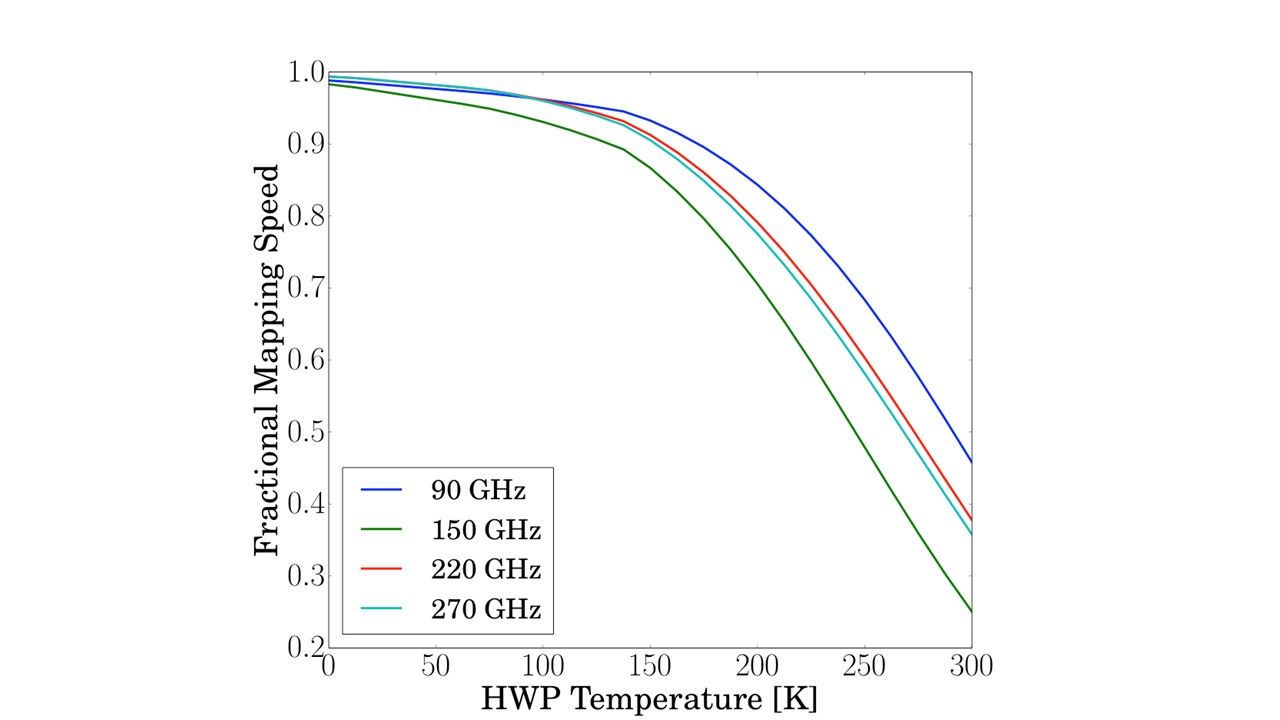
\includegraphics[width=0.98\linewidth]{CHWPDesign/Figures/chwp_mapping_speed.jpg}
    \caption[The impact of a cryogenic half-wave plate on instrument mapping speed]{The fractional impact on mapping speed---which is a quantification of the instrument white-noise level---of a three-stack achromatic HWP vs its temperature, compared to the scenario of no HWP, in the 90, 150, 220, and 270 GHz observation bands. The WHWP operates at $\sim$ 280 K, which corresponds to $\sim$ 50\% decrease in mapping speed. The CHWP, on the other hand, which operates < 100 K, corresponds to only a $\sim$ 10\% decrease in mapping speed. This sharp difference makes the cryogenic HWP a lucrative polarization modulator, as it suppresses low-frequency noise while only marginally increasing the noise floor.}
    \label{fig:chwp_mapping_speed}
\end{figure}

\begin{figure}[ht!]
    \centering
    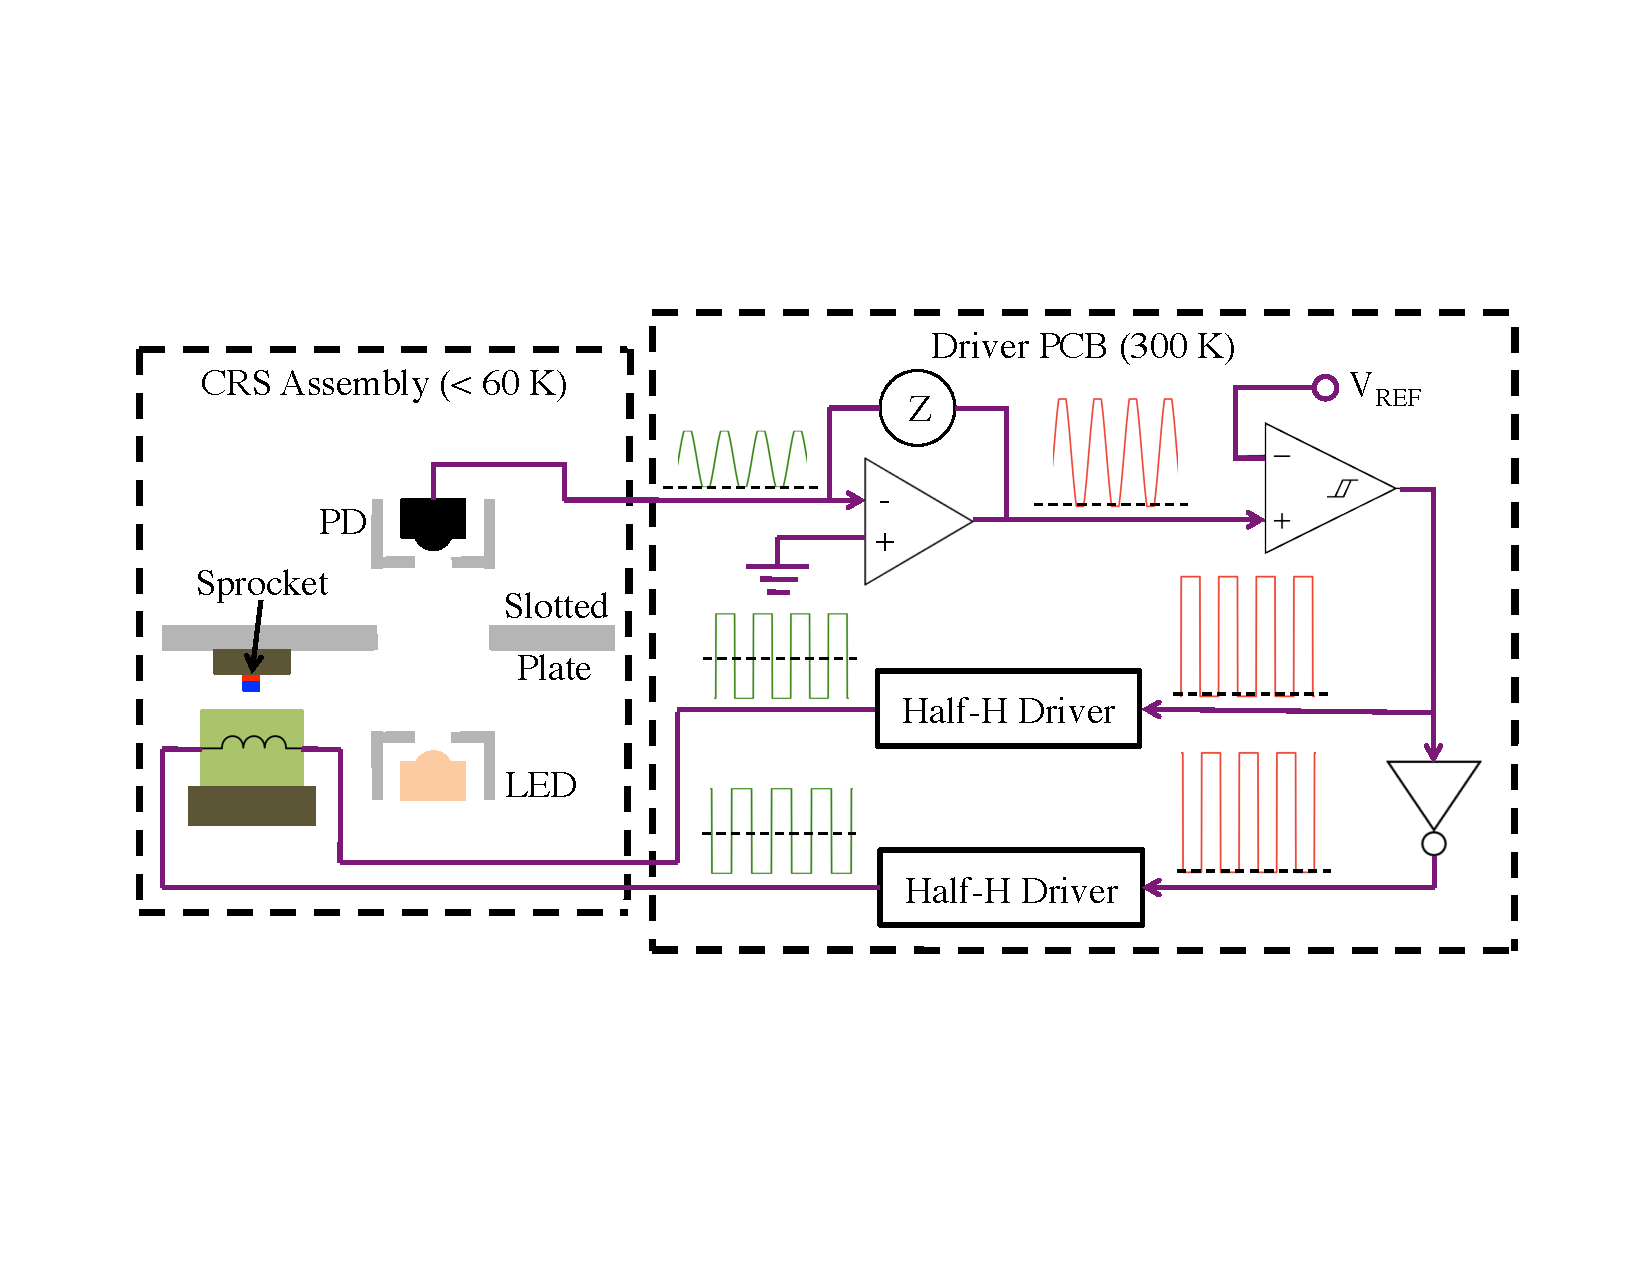
\includegraphics[width=0.98\linewidth]{CHWPDesign/Figures/MotorDiagram.pdf}
    \caption[A block diagram of one phase of the motor driver]{A block diagram of one phase of the motor driver. A current-biased, collimated LED shines onto a collimated, reverse-biased photodiode (PD) though a lane of slots on the rotor. The photocurrent signal (green) is amplified to a voltage signal (red), is referenced to a comparator voltage VREF to generate a TTL waveform, and is inverted. The inverted and non-inverted voltage signals are sent to two Half-H-bridge driver integrated circuits which are in series with the solenoid, creating a Full-H-bridge motor circuit. When the rotor rotates, the slots create an optically-chopped input to the photodiode, which the driver uses to generate an alternating current in the solenoid. The AC excitation creates an alternating magnetic field that couples to the sprockets on the rotor and hence generates torque.}
    \label{fig:chwp_motor_diagram}
\end{figure}

\begin{figure}[!ht]
    \centering
    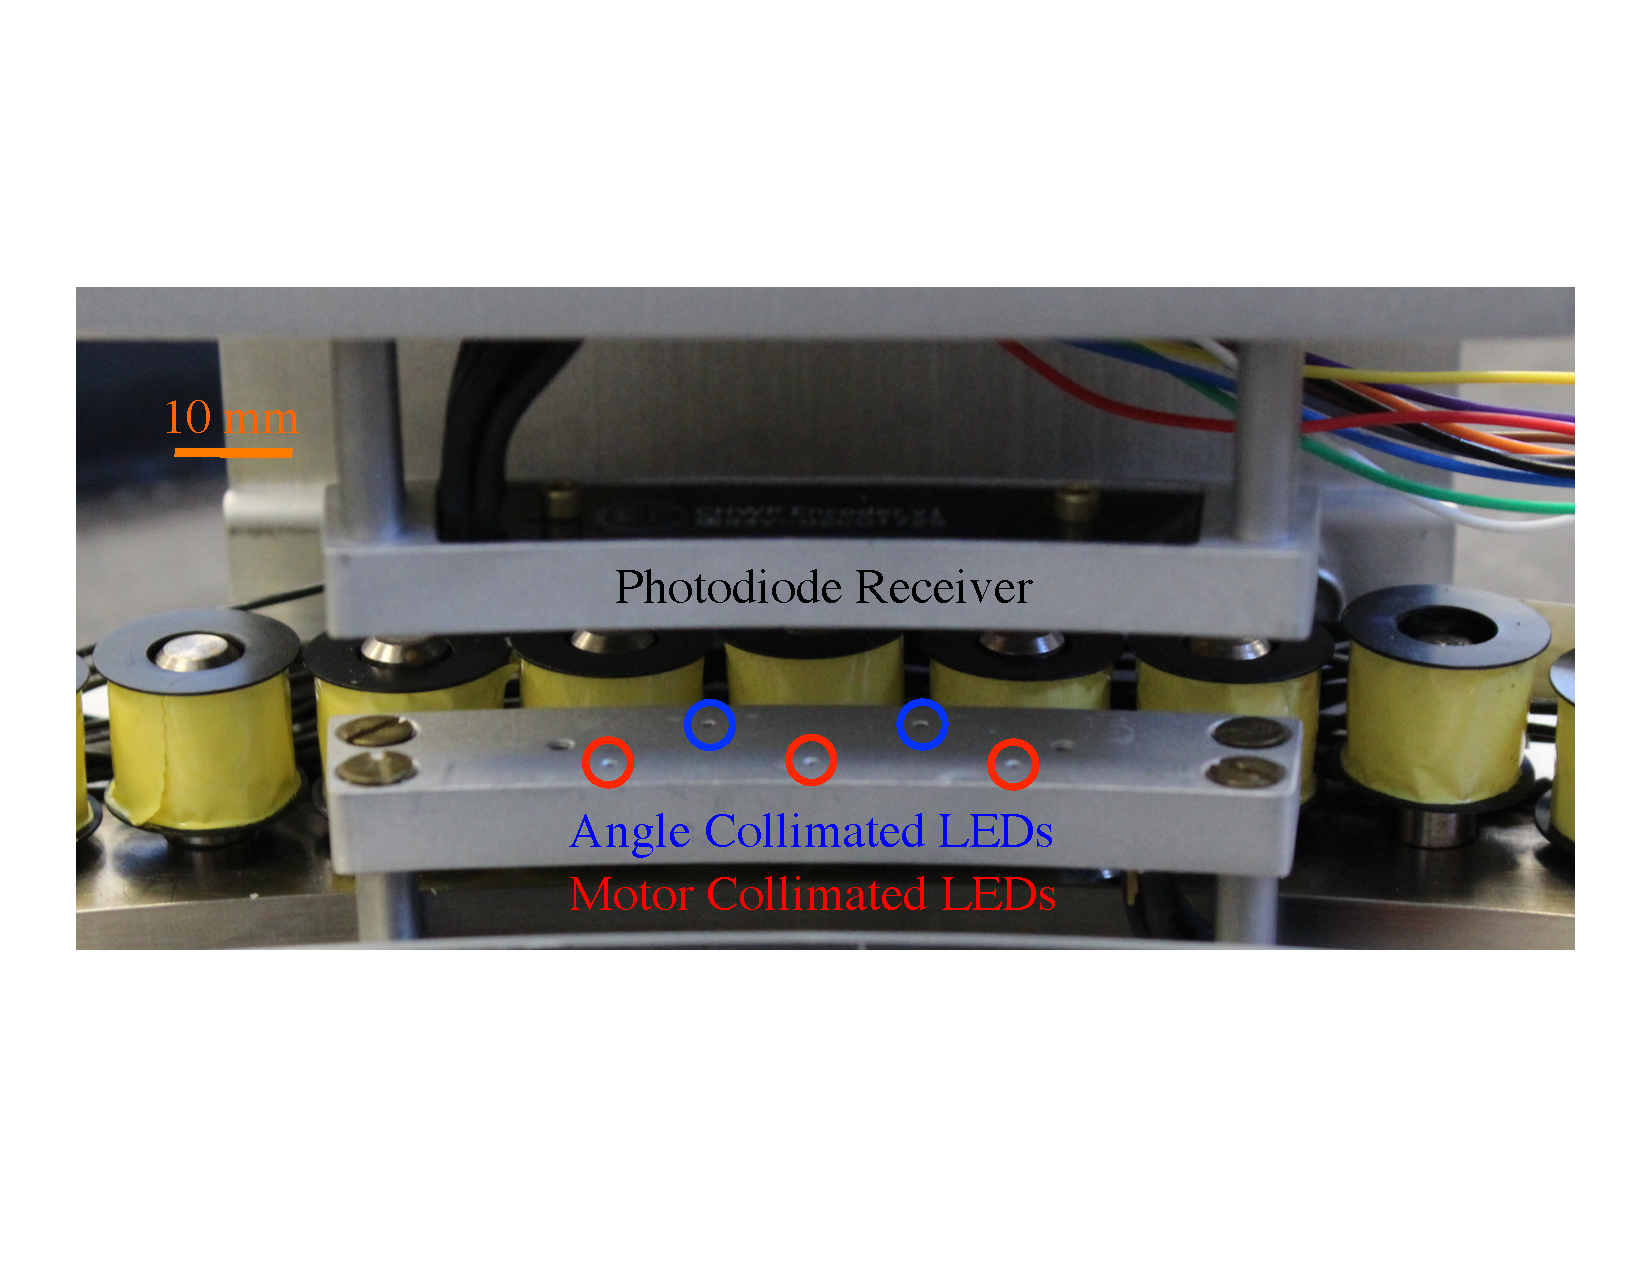
\includegraphics[width=0.6\linewidth]{CHWPDesign/Figures/Encoder.pdf}
    \caption[Photograph of the CHWP optical encoder]{The optical encoder read head and highlights which photodiode-LED pairs are used for motor and angle encoding. The motor encoder waveform is generated by a lane of coarse-resolution slots in the slotted encoder plate shown in Figure 1a, while the angle encoder waveform is generated by a lane of fine-resolution slots. Two encoder read heads are deployed for redundancy in case of an LED or photodiode failure.}
    \label{fig:chwp_encoder}
\end{figure}

\begin{figure}
    \subfloat[\label{fig:chwp_assembly:a}]{
        \raisebox{1cm}{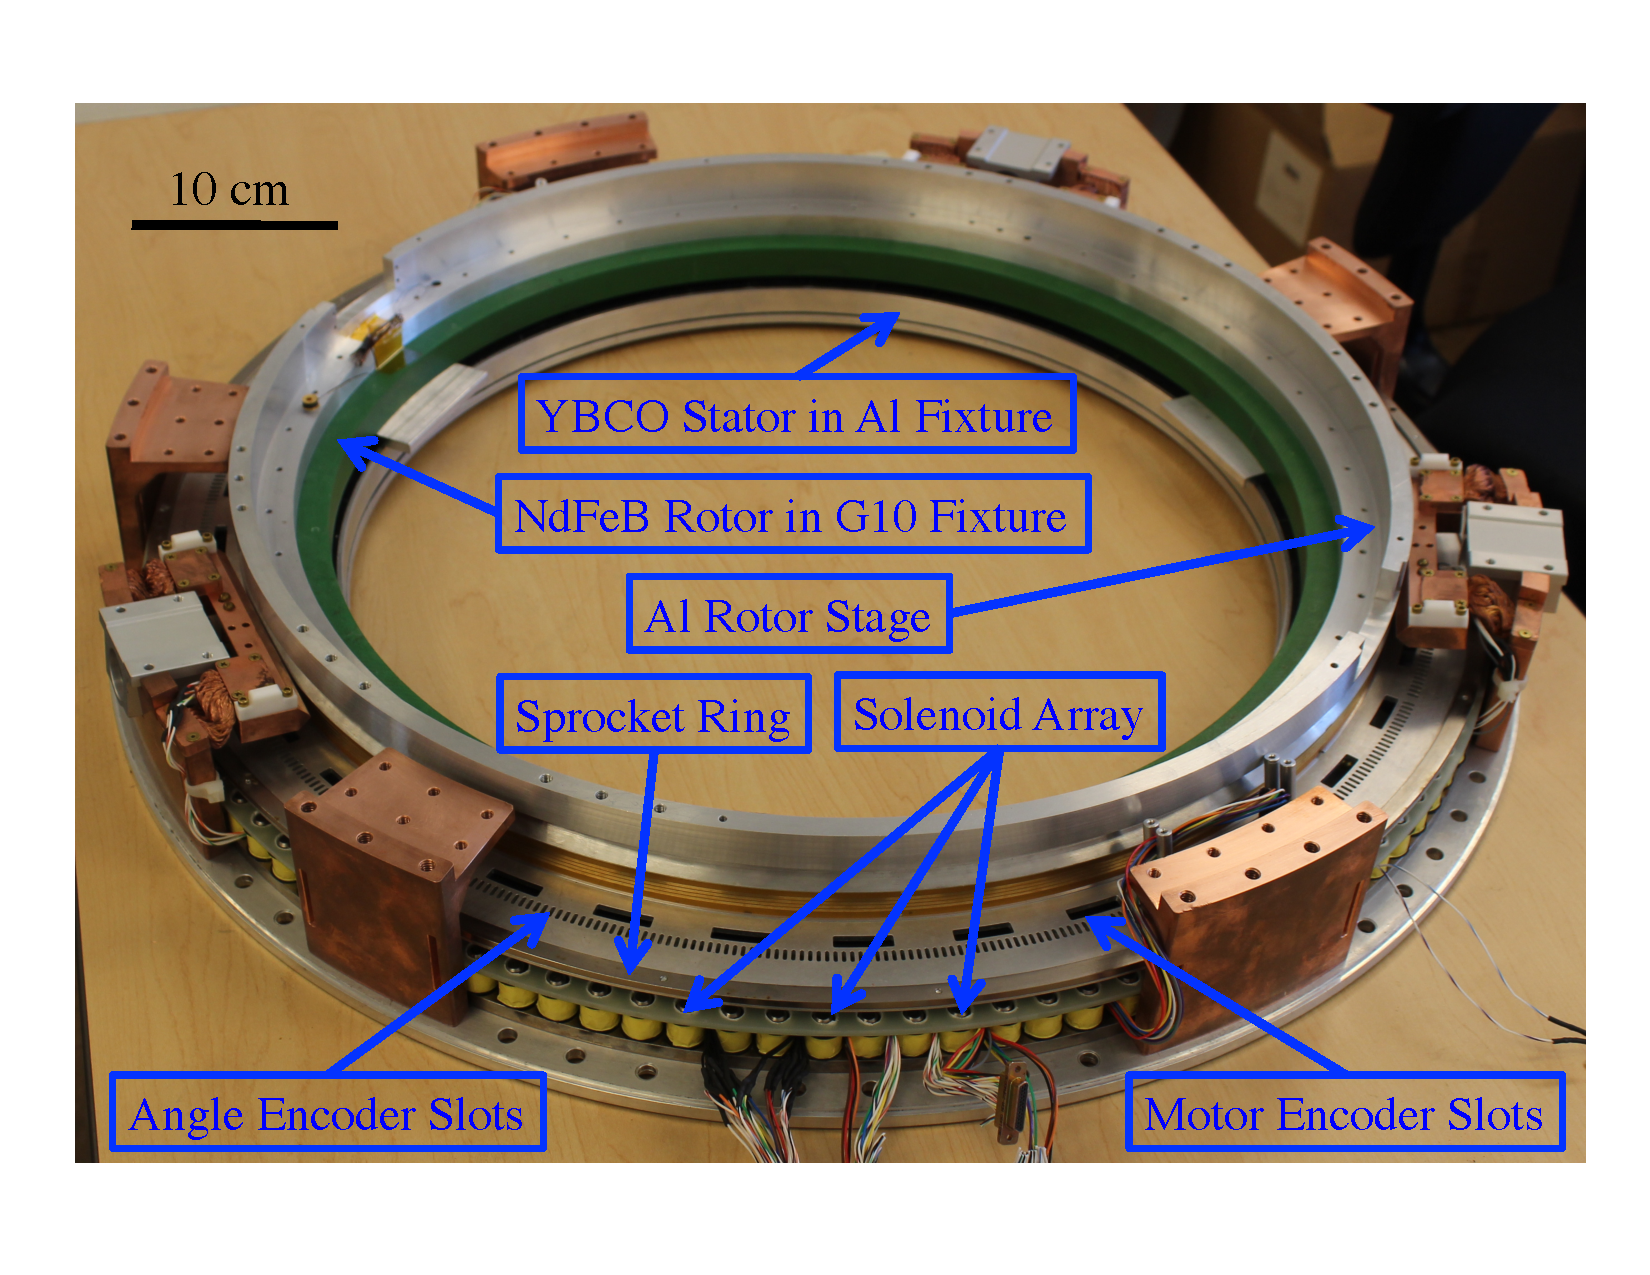
\includegraphics[width=0.48\linewidth]{CHWPDesign/Figures/RotorStator.pdf}}
    }
    \subfloat[\label{fig:chwp_assembly:b}]{
        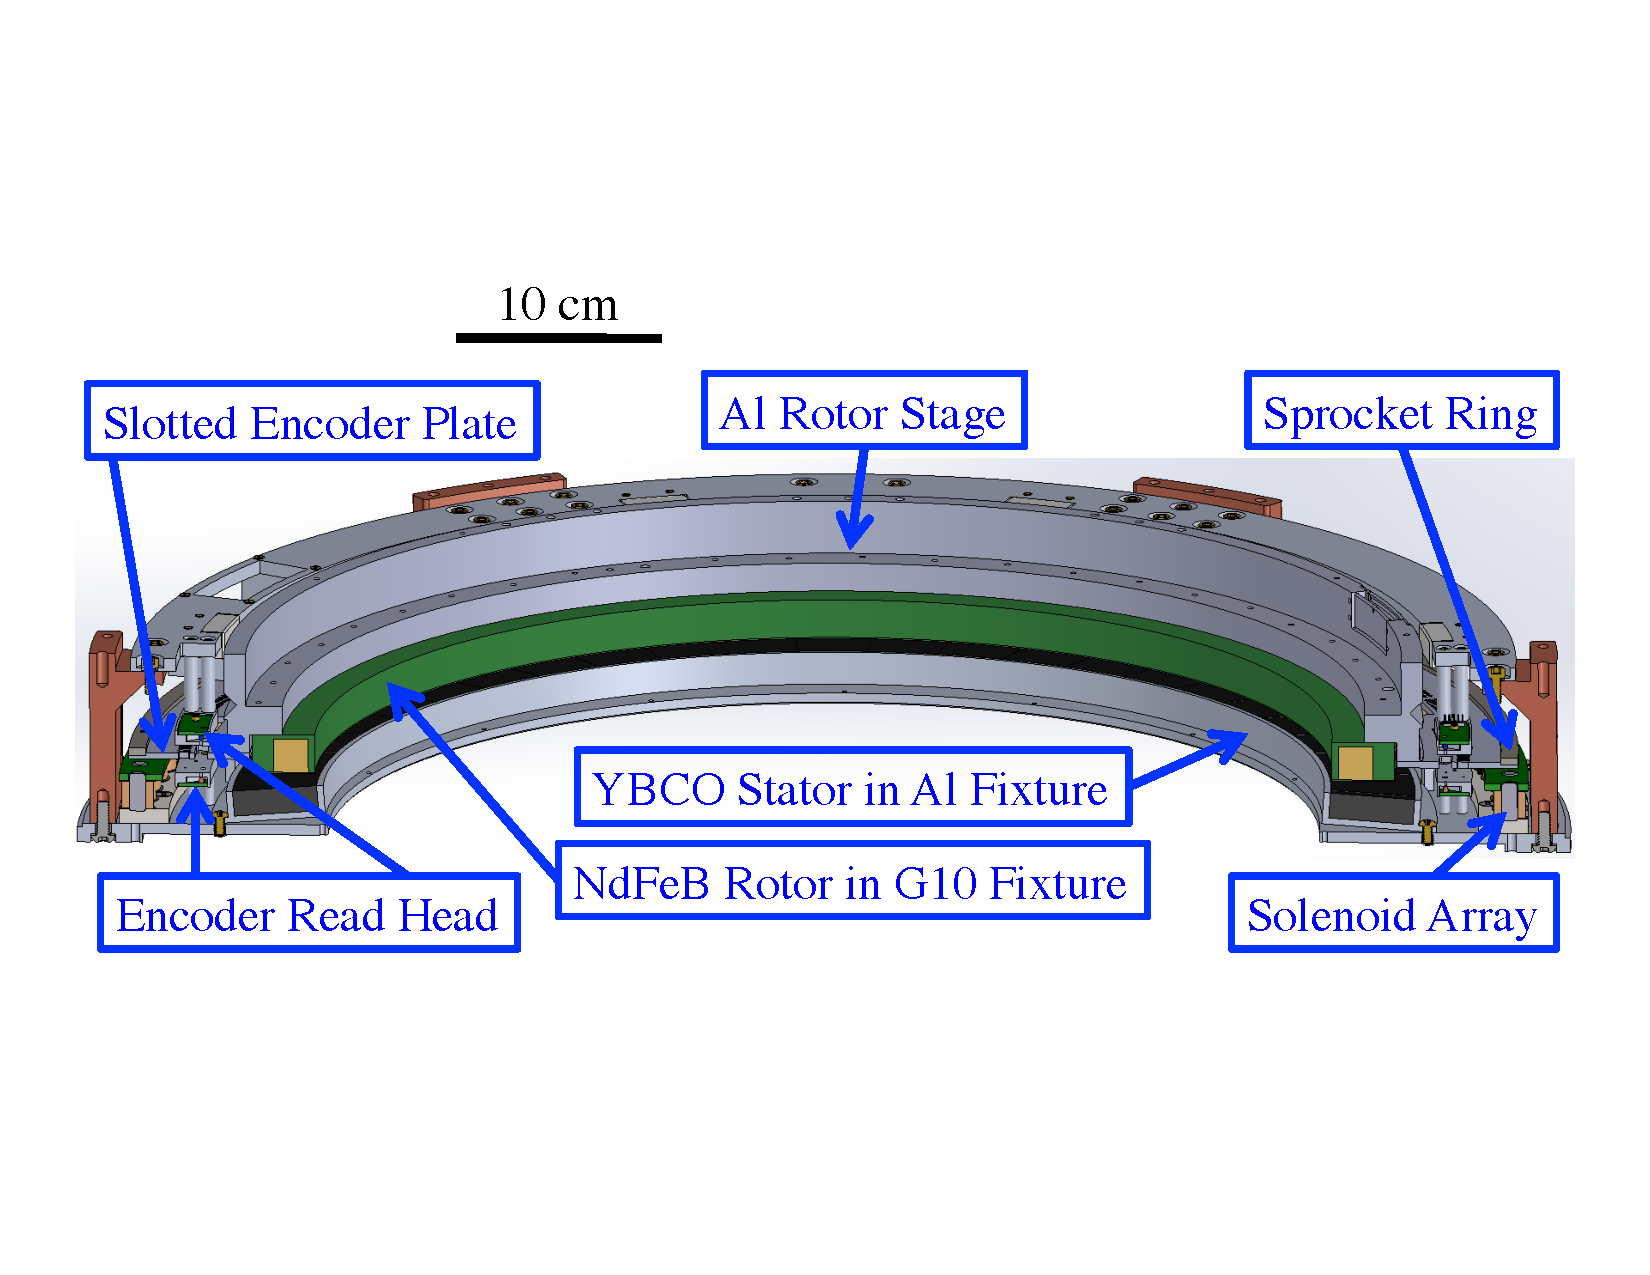
\includegraphics[width=0.48\linewidth]{CHWPDesign/Figures/StandaloneCS.pdf}
    }
    \caption[Photograph and cross section of the CHWP assembly]{Photograph and cross section of the CHWP assembly. \ref{fig:chwp_assembly:a} shows a photograph of the CHWP cryogenic assembly before being mounted in the cryostat, with key hardware elements highlighted. \ref{fig:chwp_assembly:b} shows a CAD cross section of the same assembly for a clearer look at how the assembly comes together. The buckling in the YBCO stator occurs when the assembly is cold and is due to differential thermal contraction between the YBCO and its aluminum fixture.}
    \label{fig:chwp_assembly}
\end{figure}

\begin{figure}[ht!]
    \centering
    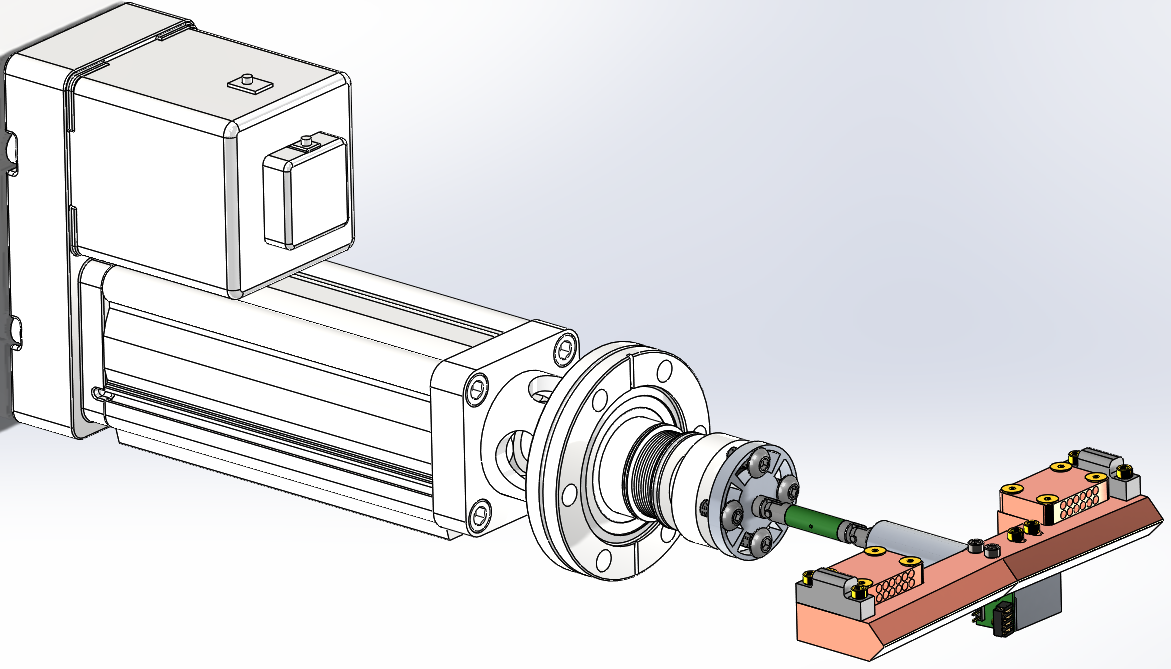
\includegraphics[width=0.98\linewidth]{CHWPDesign/Figures/Gripper_arm.png}
    \caption[CAD capture of CHWP gripper arm]{CAD capture of CHWP gripper arm. The motor assembly consists of a CF vacuum flange which mates to the cryostat vacuum shell. The stage for the motor feedthrough is then attached to a hinged thermal isolation arm made of hollow G10 fiberglass. This piece is attached to a precision-machined rod which is constrained to slide within a Frelon-lined linear bearing on the 50 K stage. In turn, this shaft is bolted to the copper gripper finger, whose wedge shape mates to a triangular groove on the CHWP rotor, hence constraining the rotor position. This particular capture is of the bottom gripper finger, which supports the weight of the rotor when warm. The wedge is angled at five degrees to keep the rotor centered in along the transverse axis.}
    \label{fig:chwp_gripper}
\end{figure}

\begin{figure}[!ht]
    \centering
    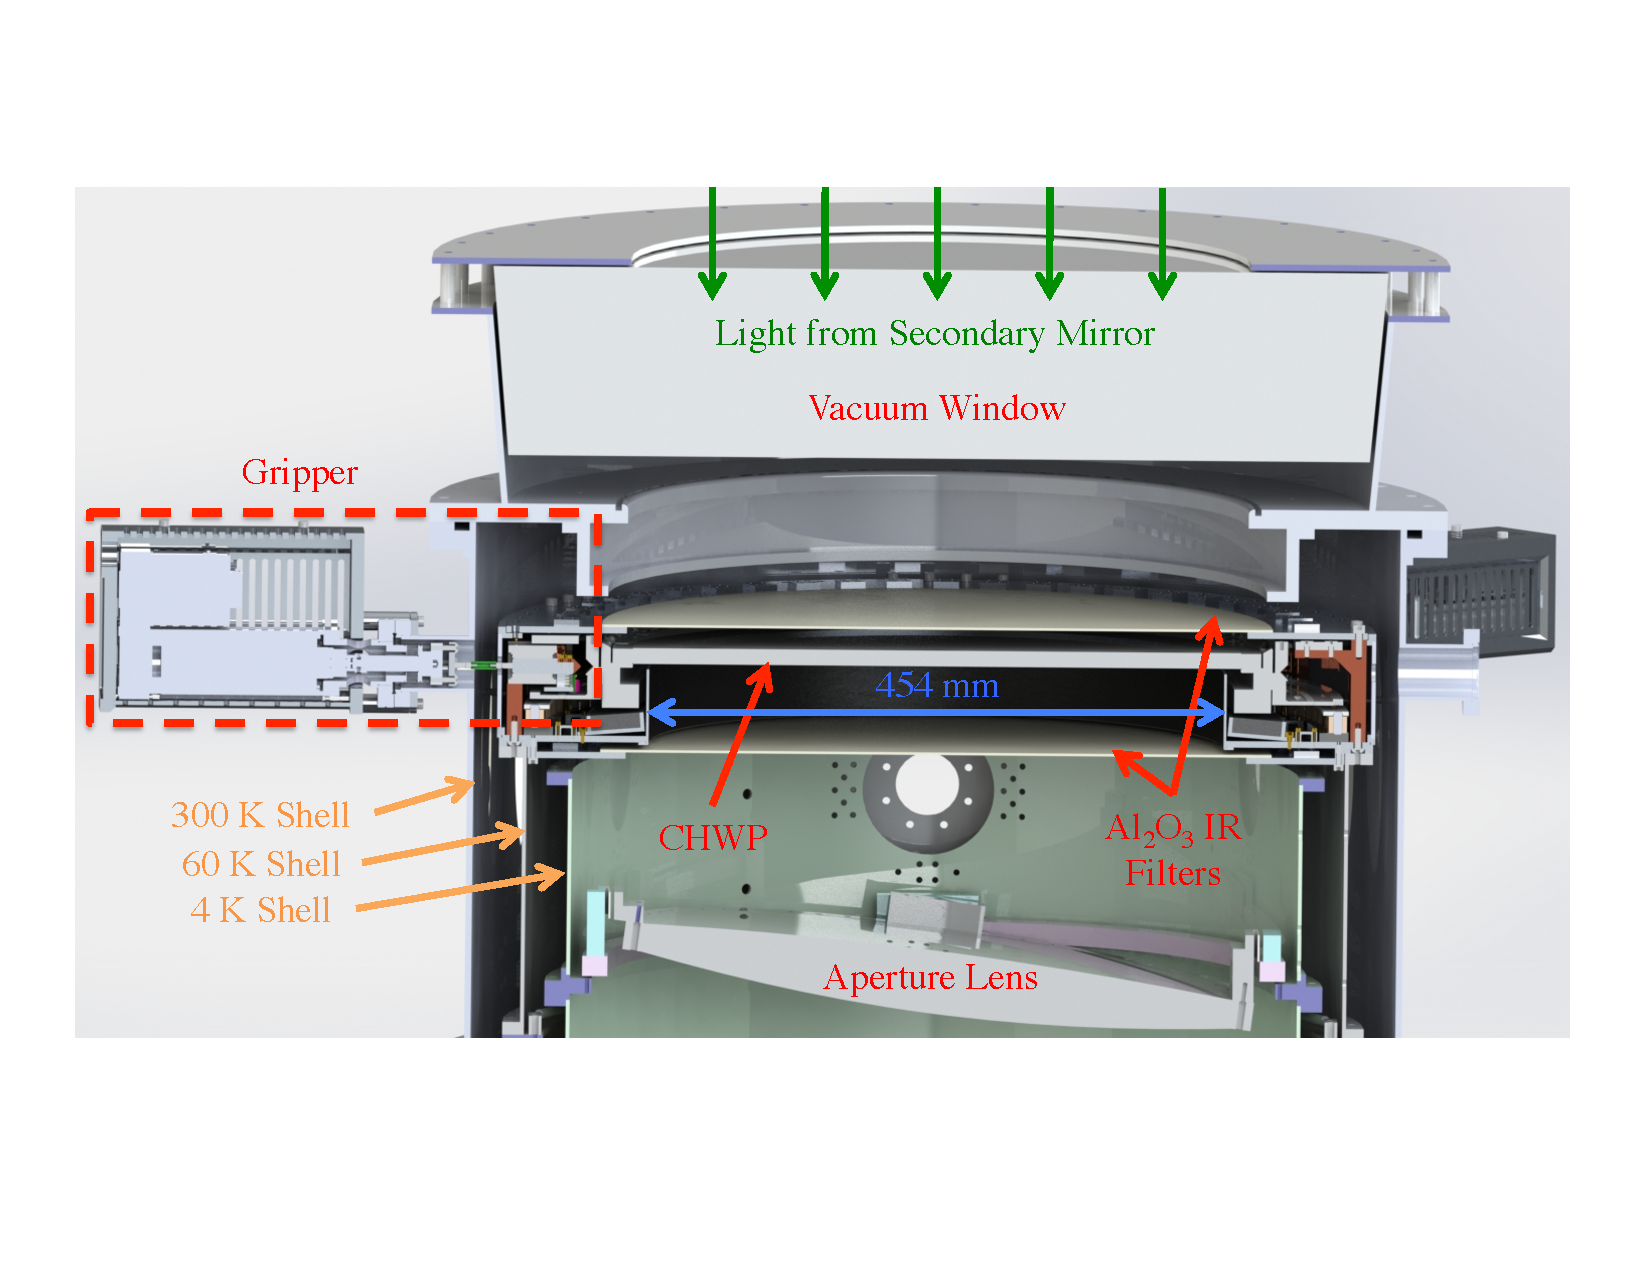
\includegraphics[width=0.6\linewidth]{CHWPDesign/Figures/PB2Implementation.pdf}
    \caption[CAD render of the CHWP inside the PB2b cryostat]{The CHWP sits inside the PB2 cryostat window at the entry to the 60 K shell, near the telescope secondary focus. It has one < 60 K alumina absorbing IR filter on either side of it to radiatively heat sink the levitating CHWP. When warm, the CHWP is aligned and held by a three-contact “gripper” system. The gripper consists of linear actuating vacuum feedthroughs, each coupled to a thermally-isolating rig, which in turn couples to a gripper “finger” in the 60 K cavity. These fingers fit into an azimuthally-cut triangular groove on the rotor, mechanically constraining the rotor while providing thermal contact for cooling. The CHWP is un-gripped in this figure.}
    \label{fig:chwp_integrated}
\end{figure}

The primary and secondary mirrors form an off-axis Gregorian configuration and create a sky image at the skyward-most field lens through a 0.5~m vacuum window. Three 4~K alumina lenses reimage onto a telecentric, 0.3~K focal plane, and a 4~K Lyot stop defines the primary mirror illumination.

\begin{figure}
    \centering
    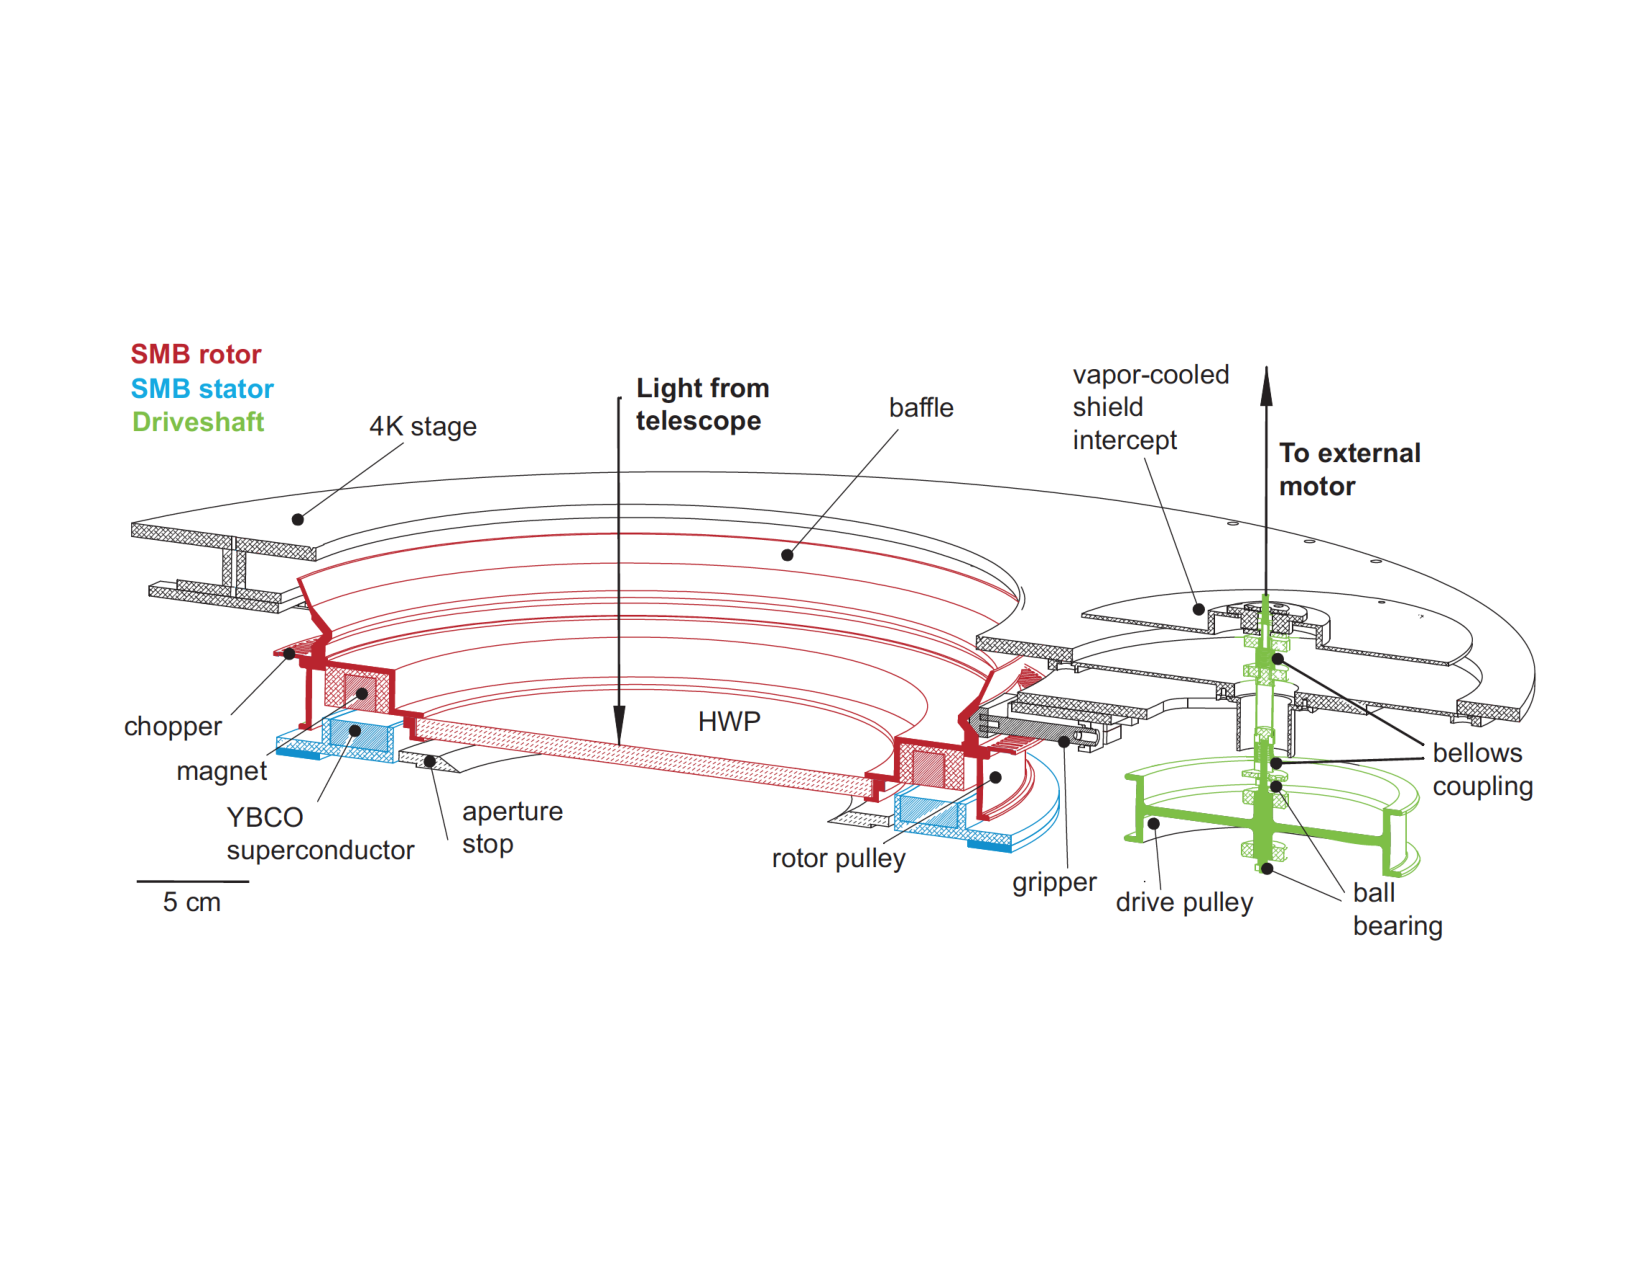
\includegraphics[width=\linewidth, trim=2cm 5cm 1.8cm 5cm, clip]{CHWPDesign/Figures/EBEX_CHWP.pdf}
    \caption{A CAD cross section of the EBEX CHWP taken from Jeff Klein's 2011 SPIE proceeding. The EBEX and PB-2b share a few key commonalities, including a superconducting magnetic bearing, a gripper, and a slot-chopped encoder. All of these systems have been upgraded in the PB-2b system, however, and several other systems, including the motor, sapphire mount, and anti-reflection coating, are totally redesigned for SA.}
    \label{fig:ebex_chwp}
\end{figure}

In this appendix, we review the details of the thermal model used in Secs.~\ref{sec:thermal_design} and~\ref{sec:temperature_stability} to simulate the rotor's equilibrium temperature, the load on the field lens, and the rotor's temperature stability.